\documentclass[10pt,a4paper]{ctexart}
\usepackage{indentfirst}
\usepackage{longtable}
\usepackage{graphicx}
\usepackage{subfigure}
\title {实验报告实验一}
\author {15231100 曹强港}
\date{}
\begin {document}
\setlength{\parindent}{2em}
\XeTeXlinebreaklocale "zh"  
\maketitle
\section{原始数据集}
\subsection{来源}
{共采集了2组数据,分别为2维数据和3维数据。}

{2维数据根据直线$2x_1+3x_2 - 4 = 0$创建,数据集中包含了200组数据,对于任意一组数据点$(x_1,x_2)$位于直线两侧,距离直线范围为$(0,10]$。数据集在记录时,添加了一维数据,成为$(x_1,x_2,(-1 | 1))$,1表示位于直线上方,-1表示位于直线下方。数据集记录在''dataset1.csv''}

{2维数据根据平面$2x_1+3x_2+ 4x_3 - 5 = 0$创建,数据集中包含了200组数据,对于任意一组数据点$(x_1,x_2,x3)$位于平面两侧,距离直线范围为$(0,10]$。数据集在记录时,添加了一维数据,成为$(x_1,x_2,x_3,(-1 | 1))$,1表示位于直线上方,-1表示位于直线下方。数据集记录在''dataset2.csv''}

\section{数据预处理}
{为了感知机算法的简化性,将二维数据中和三维数据中位于下方的数据点$(x_1,x_2,-1)$和$(y_1,y_2,y_3,-1)$转换为$(-x_1,-x_2,1)$和$(-y_1,-y_2,-y_3,1)$}
\section{实验步骤}
{1.初始化weight vector $\hat{W}$(0)。二维数据的实验中,初始化为(0,5,20);三维数据的实验中,初始化为(0,5,20,45) }

{2.利用感知机算法进行迭代,每一次迭代中每一个错误分类的数据点均会对$\hat{W}$产生影响。每隔10或100迭代次数,记录一次当前迭代中错误分类的数据点个数。}

{3.设置不同的学习率为0.01,0.1,0.2,0.3,...,0.9,0.99,分别记录步骤二中的数据,并记录不同学习率下收敛时的迭代次数和得到的直线方程(r $\hat{W}$)。}

{4.对二维数据集和三维数据集,都进行步骤1到步骤3的操作,记录并分析数据。}

\section{实验数据}
\subsection{数据集1}
\subsubsection*{迭代次数}
\begin{longtable}{|c|c|c|}
	\hline 学习率&迭代次数&向量(已处理)\\
	\hline 0.01&1645&(-2.244471848,-3.381655343,4)\\
	\hline 0.1&1479&(-2.251570102,-3.393645026,4)\\
	\hline 0.2&1541&(-2.24924311,-3.389998459,4)\\
	\hline 0.3&1536&(-2.24983023,-3.391170643,4)\\
	\hline 0.4&1550&(-2.24555108,-3.38459983,4)\\
	\hline 0.5&1577&(-2.250315653,-3.391966728,4)\\
	\hline 0.6&1558&(-2.248698272,-3.389340623,4)\\
	\hline 0.7&1569&(-2.247384684,-3.387281908,4)\\
	\hline 0.8&1562&(-2.249579796,-3.39060821,4)\\
	\hline 0.9&1562&(-2.249351384,-3.390192555,4)\\
	\hline 0.99&1550&(-2.242391559,-3.379749671,4)\\
	\hline 
	\end{longtable}
\begin{figure}[htbp]
  \centering
  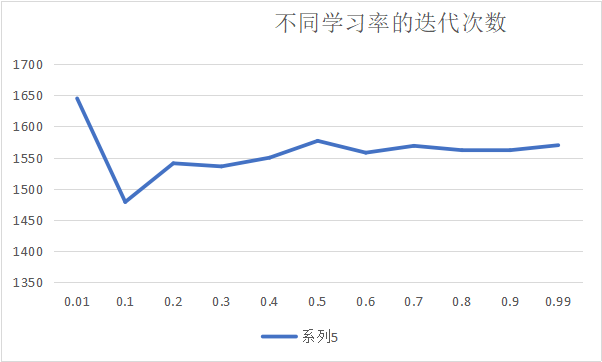
\includegraphics[width=1\textwidth]{迭代次数.png}
\end{figure}
  \subsubsection*{错误分类个数随迭代次数的变化}
  
  \begin{figure}[htbp]
  \centering
  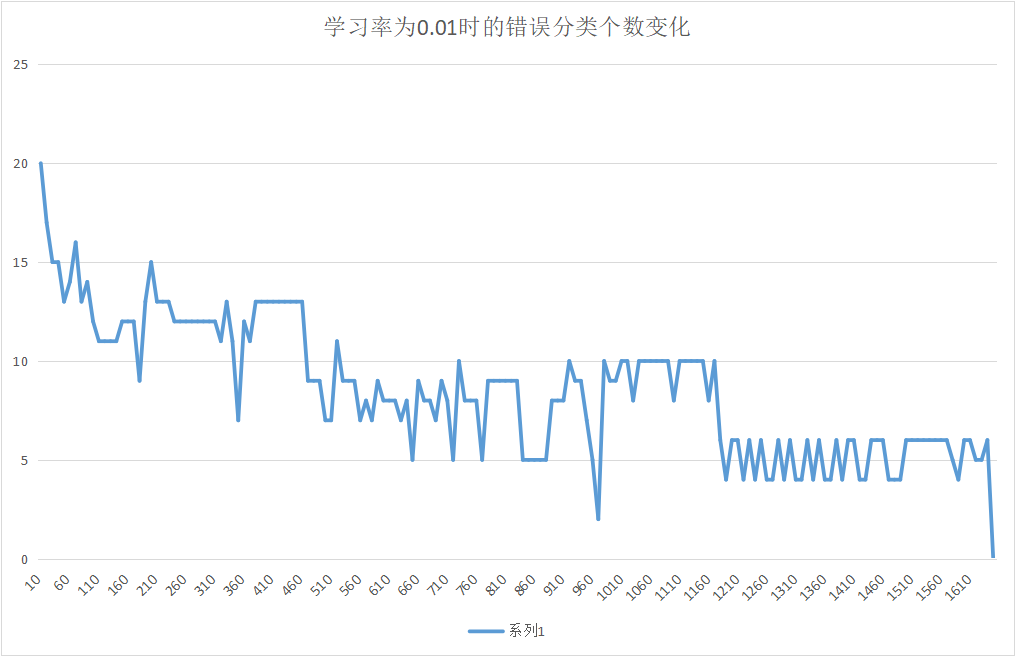
\includegraphics[width=1\textwidth]{0.01.png}
  \end{figure}
    \begin{figure}[htbp]
  \centering
  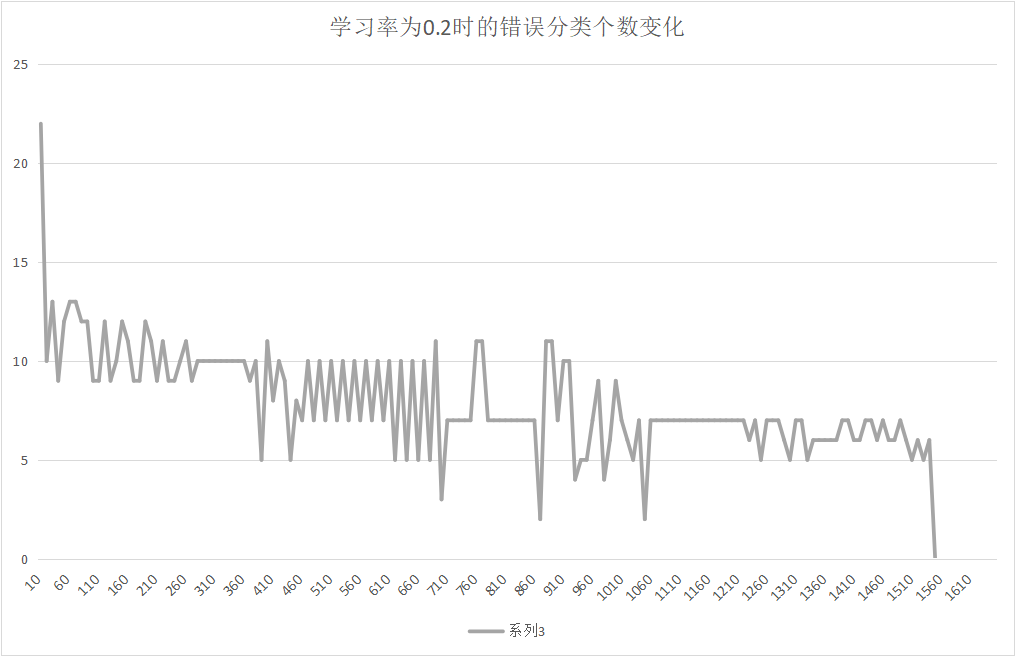
\includegraphics[width=1\textwidth]{0.2.png}
    \end{figure}
    \begin{figure}[htbp]
  \centering
  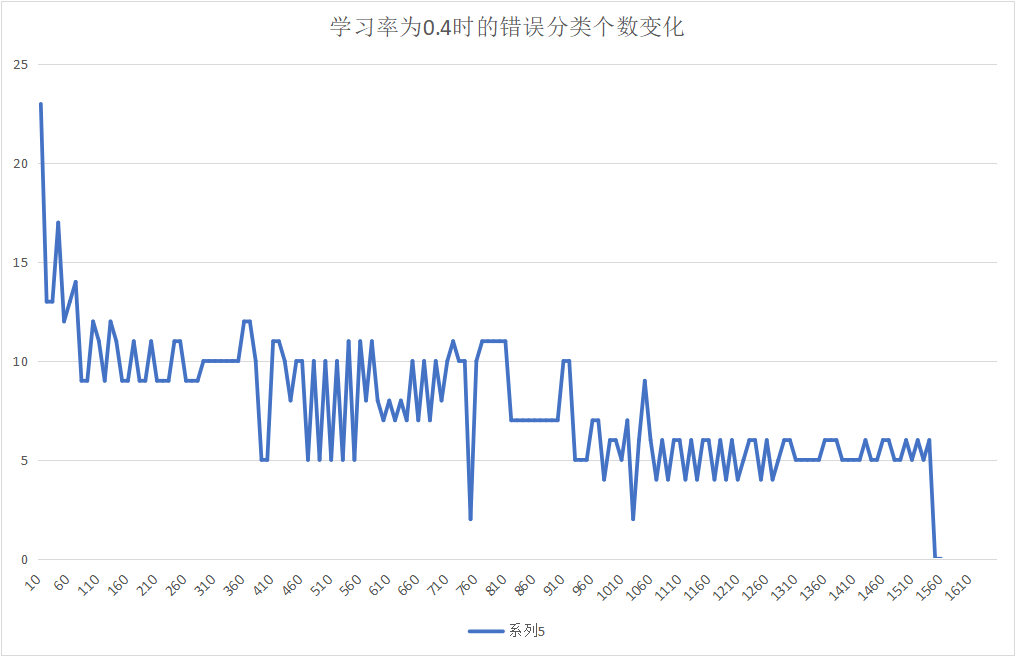
\includegraphics[width=1\textwidth]{0.4.png}
    \end{figure}
    \begin{figure}[htbp]
  \centering
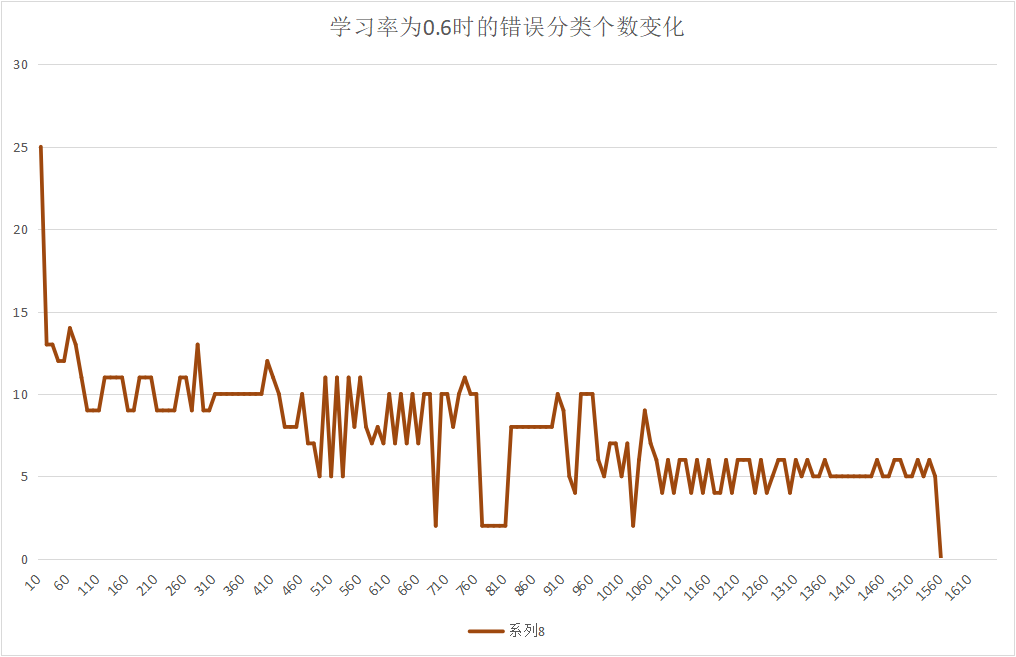
\includegraphics[width=1\textwidth]{0.6.png}
  \end{figure}
    \begin{figure}[htbp]
  \centering
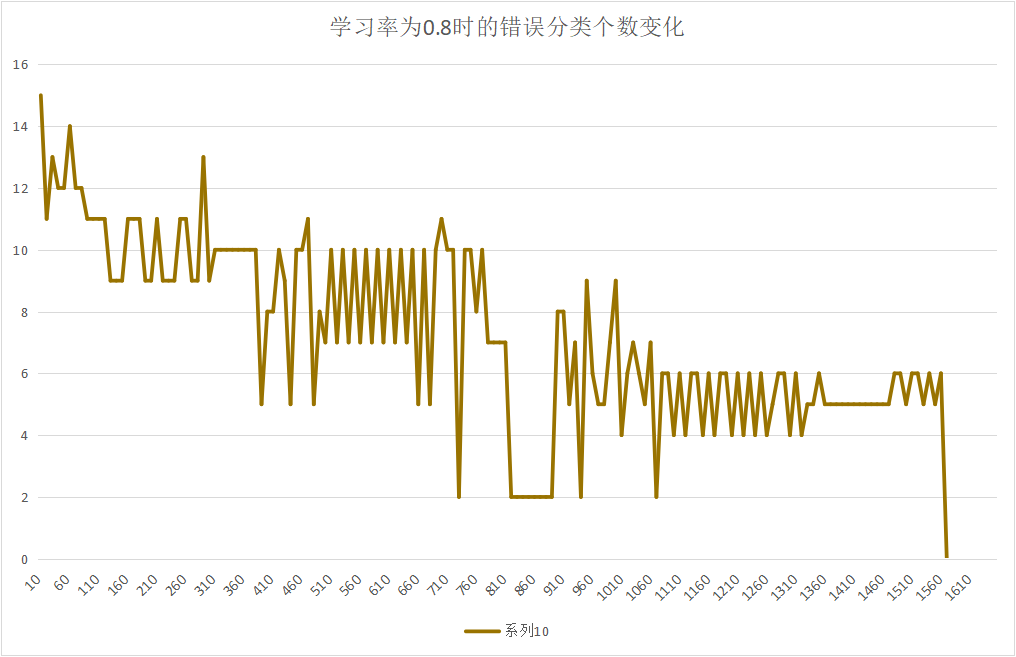
\includegraphics[width=1\textwidth]{0.8.png}
  \end{figure}
    \begin{figure}[htbp]
  \centering
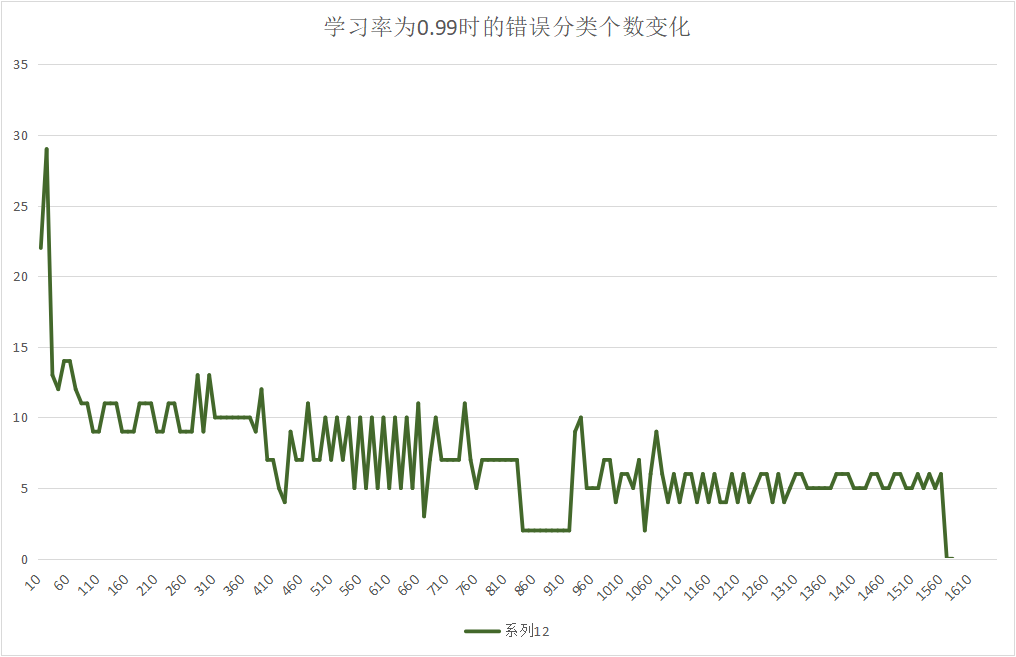
\includegraphics[width=1\textwidth]{0.99.png}
\end{figure}
\newpage
\subsection{数据集2}
\subsubsection*{迭代次数}
\begin{longtable}{|c|c|c|}
	\hline 学习率&迭代次数&向量(已处理)\\
	\hline 0.01&7044&(1.942167763,2.991252798,3.919304133,-5)\\
\hline 0.1	&6899&(1.935799178,2.978850037,3.905652123,-5)\\	
\hline 0.2	&7007&(1.94221003,2.990710071,3.919053093,-5)\\
\hline 0.3	&203890&(1.994767722,3.031921564,3.999931218,-5)\\	
\hline 0.4	&201195&(1.995396729,3.033231016,4.001340657,-5)\\	
\hline 0.5	&201700&(1.995074649,3.032444268,4.000563569,-5)\\	
\hline 0.6	&200947&(1.995453479,3.033217345,4.00139915,-5)\\	
\hline 0.7	&40252&(2.005733815,3.033692721,4.016678797,-5)\\	
\hline 0.8	&6971&(1.937408701,2.987559465,3.911967239,-5)\\	
\hline 0.9	&44002&(2.006672689,3.029927748,4.016781729,-5)\\	
\hline 0.99&203375&(1.995493868,3.033289313,4.001494139,-5)\\
	\hline 
	\end{longtable}
\begin{figure}[htbp]
  \centering
  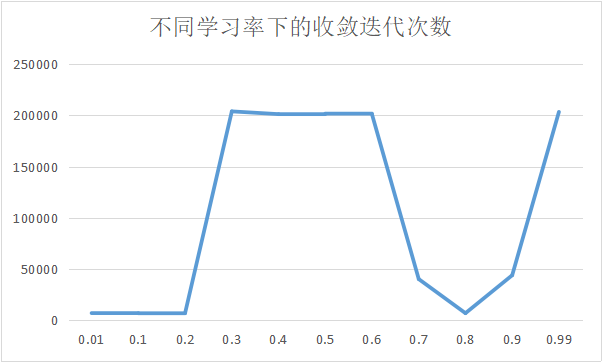
\includegraphics[width=1\textwidth]{迭代次数2.png}
\end{figure}
  \subsubsection*{错误分类个数随迭代次数的变化}
  
  \begin{figure}[htbp]
  \centering
  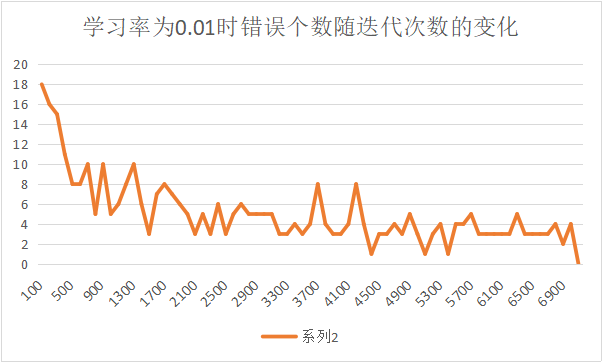
\includegraphics[width=1\textwidth]{1.01.png}
  \end{figure}
    \begin{figure}[htbp]
  \centering
  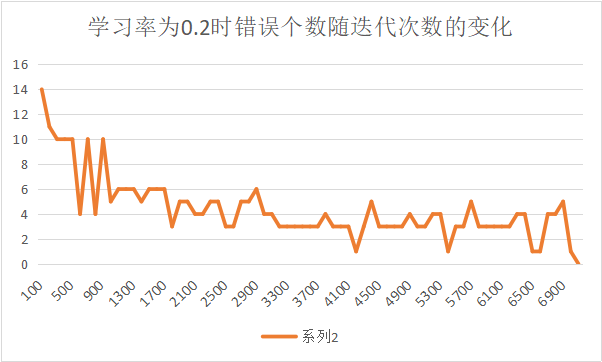
\includegraphics[width=1\textwidth]{1.02.png}
    \end{figure}
    \begin{figure}[htbp]
  \centering
  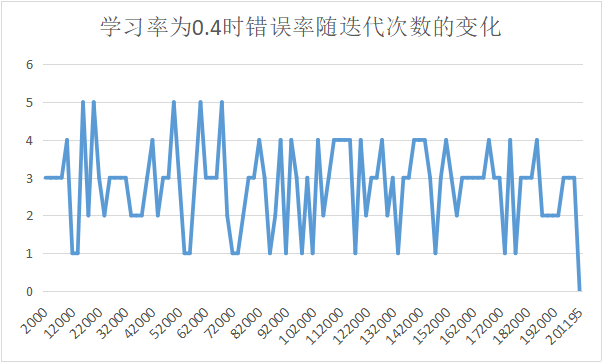
\includegraphics[width=1\textwidth]{1.04.png}
    \end{figure}
    \begin{figure}[htbp]
  \centering
  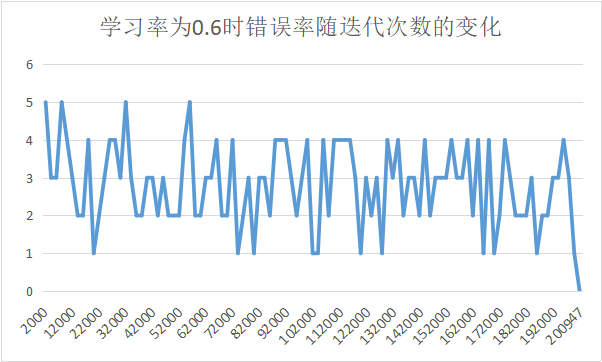
\includegraphics[width=1\textwidth]{1.06.png}
    \end{figure}
    \begin{figure}[htbp]
  \centering
  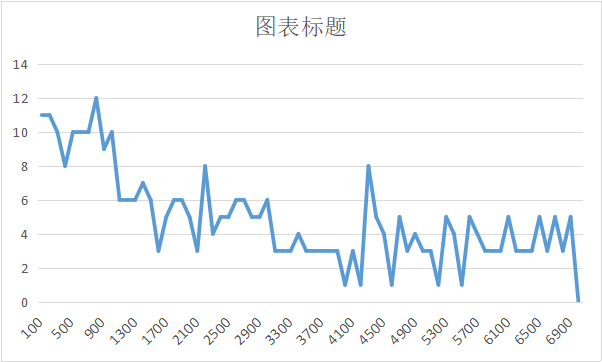
\includegraphics[width=1\textwidth]{1.08.png}
    \end{figure}
    \begin{figure}[htbp]
  \centering
  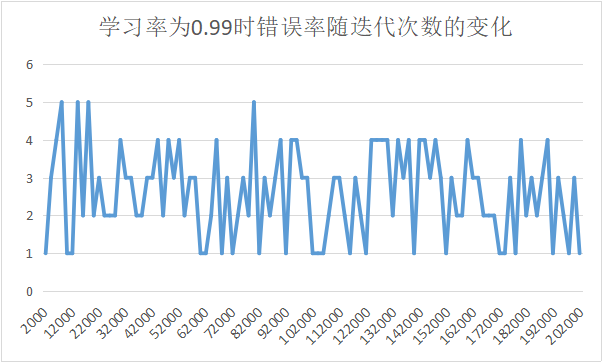
\includegraphics[width=1\textwidth]{1.99.png}
    \end{figure}

\newpage
\section{实验分析}
\subsection{现象和结论}
  {1.观察可知,当学习率逐渐由小增大时,感知机收敛时的迭代次数会随之先减后增}
  
  {2.在某些较大的学习率的情况下,迭代次数会突然达到较高的数量级。此时梯度下降的值较大,很难正好达到收敛。}
  
  {3.支持向量的初始值对总的迭代次数有影响,特别的,当初始值为零向量时,迭代次数与学习率无关}
  
  {4.错误分类的个数最初会随着迭代次数的增加而减少,学习率越高时减少越明显;然后可能会出现震荡(忽高忽低),学习率越高时震荡的幅度越大,越难达到收敛}
  
  {5.学习率越低或者越高并不一定能取得最优解,因为损失函数只是判别是否有数据点被分错,不关心所有分类的点是否与分类面相距较远(``分得越开'')}
  \section{代码以及相关数据}
  {代码可在找到}
\end {document}